\chapter{Selection Bias Removal}
\label{ch-sb-removal}
This chapter
is based on Ref.\cite{bare-sb-removal}.

Selection bias (SB)
occurs when one
samples from an
atypical subset
of a
population,
producing a biased dataset.
Are such biased
datasets
useless? Not necessarily.
It is possible to
add auxiliary features
to the biased dataset, and to
sample those new features
in an unbiased way,
 from the whole population.
Then
one can merge
the original
 biased dataset with the
auxiliary, unbiased one,
to obtain an enhanced dataset.
It is sometimes
possible to do this so that the enhanced
dataset is provably
unbiased.
It's like making horizontal
the surface of a table
 that was
 not initially
horizontal.
The theory of Bayesian Networks and Causal
Inference tells us
WHEN this is possible,
and HOW to do it
when it is possible.


\section{Root and Leaf Nodes}

Root and Leaf (R-L) nodes play an important role in many facets of
bnet theory. In this section, we will review what we know
about them from previous chapters in this book, and then we will add a few new
ideas like R-L conversion and R-L selectors.

A root node selects a different bnet 
for each of its values.
Root nodes are used
in Chapter \ref{ch-transport}
entitled \qt{Transportability
of Causal Knowledge}
as bnet switches (i.e., bnet selectors).




\begin{figure}[h!]
\centering
\includegraphics[width=1in]
{sb-removal/common-cause-effect.png}
\caption{Common Cause
and Common Effect for
treatment node $\rvd$
and outcome node $\rvy$.}
\label{fig-common-cause-effect}
\end{figure}

In Potential
Outcomes (PO) theory
 (see Chapter \ref{ch-pot-out}),
root nodes such
as $\rva$ in
Fig.\ref{fig-common-cause-effect}
are called {\bf common cause
 (a.k.a. confounder, fork) nodes}
for the treatment node $\rvd$
and outcome node $\rvy$.
In PO theory, leaf nodes such as
$\rvb$ in
Fig.\ref{fig-common-cause-effect} are
called
{\bf common effect
(a.k.a. selection bias (SB), collider) nodes
for nodes $\rvd, \rvy$}.
Hence, in PO theory,
SB is indicated
by
a leaf node,
just as we do in this chapter.

Note that
{\bf Simpson's paradox} (see Chapter
\ref{ch-simpson}) arises from an indirect effect
caused by \ul{not conditioning}
on a confounder,
whereas
{\bf Berkson's paradox}
(see Chapter \ref{ch-berkson})
arises from an indirect effect
caused by \ul{conditioning}
on a collider.

\subsection{R-L Conversion}

It's possible to replace a root node
by a leaf node, or vice versa, as
follows.
Suppose that we start with
a bnet $G_0$ that is \ul{fully connected}, and
we add to it a node $\rvbeta$
that is a root node that points
to all nodes of $G_0$.
Call the resulting bnet $\rvbeta\rarrow G_0$.
We can use Bayes rule to reverse the direction
of the arrows emanating from $\rvbeta$
so that they enter node $\rvbeta$
rather than exit
it.
Call the resulting bnet $\rvbeta\larrow G_0$.
In general,
Bayes rule allows us to translate
from $\rvbeta\rarrow G_0$ to
$\rvbeta\larrow G_0$,
or in the opposite direction,
without having to change the
directions of any of the arrows in $G_0$.
If $G_0$ is not fully connected, then
going from root-$\rvbeta$,
$\rvbeta\rarrow G_0$, to leaf-$\rvbeta$,
$\rvbeta\larrow G_0'$,
will often require that $G_0'$
have the same arrows in the same
directions as $G_0$
plus some extra arrows
new to $G_0$.
Likewise, going
from leaf-$\rvbeta$, $\rvbeta\larrow G_0$, to root-$\rvbeta$,
$\rvbeta\rarrow G_0''$,
may require that $G_0''$ have
the same arrows as $G_0$ plus some new arrows.

So far, we have
been intentionally
vague in specifying the graphs
$G_0'$ and $G_0''$.
In Fig.\ref{fig-sel-nd-reversal}
we give a trick for determining
possible candidates for
graphs $G_0'$ and $G_0''$.
In
Fig.\ref{fig-sel-nd-reversal},
we consider 3 panels going from left
to right, depicting
the cases where $\rvbeta$ has either 1,2 or 3 neighbors.
The top graph
 $G_{leaf}$, which has
a leaf $\rvbeta$, is converted
to a graph which is numerically
equal to it, namely
the bottom
graph
 $G_{root}$, which has
a root $\rvbeta$.
The magenta arrows represent
any number of arrows
exiting (but none entering)
a node.

If we start
with a graph $\rvbeta\larrow G_0$,
we find the biggest subgraph $X$ of
$G_0$ such
that $\rvbeta\larrow X$ only has nodes
exiting it (i.e., only magenta nodes).
Then we add enough
arrows to $\rvbeta\larrow X$
to make it a fully connected graph
$\rvbeta\larrow X'$.
Now we can reverse the incoming
arrows to $\rvbeta$ and make them
all outgoing and call the
resulting graph $\rvbeta\rarrow X'$.

A fully connected subgraph of 
a graph $G_0$ is called a 
{\bf clique} of $G_0$.
I like to call a subgraph $X$  of $G_0$ that only has exiting arrows, an 
{\bf exploding subgraph}.



\begin{figure}[h!]
\centering
\includegraphics[width=4in]
{sb-removal/sel-nd-reversal.png}
\caption{Converting 
a leaf node
to a root node.}
\label{fig-sel-nd-reversal}
\end{figure}

Recall that in Chapter \ref{ch-bnet-def},
we made a distinction
between a good Causal Fit (CF) bnet
a bad CF bnet, and
we pointed out
that bad CF bnets are
often useful as
numerical tools.
Recall also from Chapter
\ref{ch-obs-equi}
that two bnets can be
\qt{observationally equivalent}.
That is what is happening here.
We are faced with
the choice of
using
either
leaf nodes or root nodes.
Both
choices  lead to observationally
equivalent bnets.
One of the two choices
leads to a good
CF bnet,
and the other to a bad CF bnet.
Both choices are numerically
correct.

\subsection{R-L selectors}
R-L selectors are nodes 
$\rvs\in \bool$ that allow us to merge 2 bnets into a single one. In this chapter they allow us 
to consider two bnets, with and without SB, at the same time.
In the case of transportability (see Chapter \ref{ch-transport}), they allow us to transport causal knowledge
between experiments.


\begin{figure}[h!]
$$
\begin{array}{ccc}
\xymatrix{
&\rvbeta\ar[dl]\ar[d]\ar[dr]&\rvs\ar[l]
\\
&&
}
&\quad\quad&
\xymatrix{
\ar[dr]&\ar[d]&\ar[dl]
\\
&\rvbeta&\rvs\ar[l]
}
\\
(a)\text{ root node selector} 
&& (b)\text{ leaf node selector}
\end{array}
$$
\caption{$(a)$ (resp., $(b)$) shows a selector node $\rvs$ for a
root node (resp., leaf node) $\rvbeta$.}
\label{fig-rl-selectors}
\end{figure}

Fig.\ref{fig-rl-selectors}
$(a)$ shows a selector node $\rvs$ for a
root node  $\rvbeta$.  In this case,
the TPM, printed in blue, of node $\rvbeta$ is                        


\beq\color{blue}
P(\rvbeta=\beta|s)=
\left\{
\begin{array}{ll}
\delta(\beta, \beta_0)&\text{if $s=0$}
\\
P^*(\beta)&\text{if $s=1$}
\end{array}
\right.
\eeq

Fig.\ref{fig-rl-selectors}
$(b)$ shows a selector node $\rvs$ for a
leaf node  $\rvbeta$.  In this case,
the TPM, printed in blue, of node $\rvbeta$ is   

\beq\color{blue}
P(\rvbeta=\beta|s, pa^-(\rvbeta))=
\left\{
\begin{array}{ll}
P(\beta)&\text{if $s=0$}
\\
P^*(\beta|pa^-(\beta))&\text{if $s=1$}
\end{array}
\right.
\eeq

\section{SB-Recoverability}

Consider the bnet
Fig.\ref{fig-bs-removal-basic}.

\begin{figure}[h!]
$$
\xymatrix{
\rvx\ar[r]\ar@{<->}[d]
&\rvy\ar@{<->}[dl]
\\
\Rect{\rvA}&\rvs\ar[l]
}
$$
\caption{Bnet considered for
selection bias (SB) removal.
Double arrows stand for any number of arrows in
either direction.}
\label{fig-bs-removal-basic}
\end{figure}

$\rvs\in \{0,1\}$ {\bf selector node}

$\rvx=$ {\bf treatment node}.

$\rvy=$ {\bf outcome node}.

$\rvA=$ {\bf auxiliary features}.
This is a set of nodes that
may contain arrows entering
or exiting it, as indicated by the double arrows.

$\rvE=\{\rvy, \rvx\}\cup\rvA=$
{\bf Enhanced feature set}.


$\Sigma=$ unbiased population of individuals $\s$

$\Sigma_o=$ biased sub-population of individuals,
$\Sigma_o\subset \Sigma$.

$OD=\{({\s_o},\rvx^{\s_o},  \rvy^{\s_o},\rvs^{\s_o}=1):{\s_o}\in\Sigma_o\}=$
{\bf Original Dataset}, dataset for $(\rvx,\rvy)$ features
with $\rvs=1$.
Gives empirical
distribution $\color{red}{P(y|x, \rvs=1)}$.
(Ref.\cite{bare-sb-removal}
calls this dataset the {\bf biased study}.)

$AD=\{(\s, \rvx^\s,\rvA^\s):\s\in\Sigma\}=$
{\bf Auxiliary Dataset}, dataset for $(\rvx, \rvA)$ features.
Gives empirical
distribution $\color{red}{P(A|x)}$.
(Ref.\cite{bare-sb-removal}
calls this dataset the
{\bf population level study}.)


$ED=\{({\s_o},\rvx^{\s_o}, \rvA^{\s_o}, \rvy^{\s_o},
\rvs^{\s_o}=1):{\s_o}\in\Sigma_o\}=$
{\bf Enhanced Dataset}, dataset for $(\rvx,\rvy, \rvA)$ features
for $\rvs=1$.
Obtained by merging $OD$ and $AD$.
Gives empirical
distribution $\color{red}{P(y|x, A, \rvs=1)}$.




\subsection{Removing SB from
passive query}

We will refer to $Q=P(y|x, a., \rvs=1)$ 
for some multinode $\rva.$\footnote{$\rva.$ may be empty.}
as a {\bf  passive query}.
A {\bf passive query is
SB-recoverable}
via $\rva.$ if $\rvy\perp\rvs|(\rvx, \rva.)$ so

\beq
P(y|x, a. \rvs=1)=P(y|x, a.)
\;.
\eeq

\begin{claim}\label{cl-sb-recov}
There exists $\rva\subset \rvA$
 such that
 $\rvy\perp\rvs|(\rvx,\rva)$
and $\rva\perp\rvs|\rvx$
iff
\beq
P(y|x, \rvs=1)
=
\sum_a
\underbrace{P(y|x, a, \rvs=1)}_
{P(y|x,a)}
\underbrace{P(a|x, \rvs=1)}_{P(a|x)}
=P(y|x)
\eeq

\beq
\xymatrix{
\rvs=1\ar[rd]
\\
x\ar[r]
&y
}
\xymatrix{\\=}
\xymatrix{
&\sum a\ar[d]
\\
x\ar[r]\ar[ru]
&y}
\xymatrix{
\\=}
\xymatrix{\\
x\ar[r]&y}
\eeq
\end{claim}
\proof

The $\Rightarrow$ part of this
claim is obvious. For a proof
of the $\Leftarrow$ part, see
 Ref.\cite{bare-sb-removal}.
\qed





\subsection{Removing SB from
active query}

We will refer to $Q=P(y|\cald \rvx=x, a., \rvs=1)$ 
for some multinode $\rva.$
as an {\bf  active query}.
An {\bf active query is
SB-recoverable}
via $\rva.$ if 

\beq
P(y|\cald \rvx = x, a., \rvs=1)=P(y|\cald \rvx = x, a.)
\;.
\eeq
                                      
\subsection{Examples}
\hrule
\begin{enumerate}
\item Selection Bias (SB)
\beq\xymatrix{
\rvx\ar[rr]\ar[dr]
&&\rvy\ar[dl]
\\
&\rvbeta&\rvs\ar[l]
}\eeq

\hrule\item Confounding
\beq\xymatrix{
&*++[F-o]{\rvbeta}
\ar[dl]\ar[dr]
&\rvs\ar[l]
\\
\rvx\ar[rr]
&&\rvy
}\eeq


\hrule\item SB of treatment.  $Q=P(y|x)$ recoverable
\beq\xymatrix{
\rvx\ar[rr]\ar[dr]
&&\rvy
\\
&\rvbeta&\rvs\ar[l]
}\eeq

\hrule\item SB of outcome. $Q=P(y|x)$ NOT recoverable
\beq\xymatrix{
\rvx\ar[rr]
&&\rvy\ar[dl]
\\
&\rvbeta&\rvs\ar[l]
}\eeq


\hrule\item $Q=P(y|x)$ recoverable
\beq\xymatrix{
\rvx\ar[rr]\ar[dr]
&&\rvy
\\
\rvz\ar[u]\ar[r]
&\rvbeta&\rvs\ar[l]
}\eeq

\hrule\item $Q=P(y|x)$ NOT recoverable
\beq\xymatrix{
&\rvw\ar[dl]\ar[dr]
\\
\rvx\ar[rr]\ar[dr]
&&\rvy
\\
\rvz\ar[u]\ar[r]
&\rvbeta&\rvs\ar[l]
}\eeq

\hrule\item $Q=P(y|\cald x=x)$ recoverable if condition on $\rvx, \rvw$
\beq\xymatrix{
\rvx\ar[dr]\ar[rr]
&&\rvy\ar[dl]
\\
&\rvw\ar[d]
\\
&\rvbeta&\rvs\ar[l]
}\eeq

\hrule\item $Q=P(y|\cald x=x)$ recoverable if condition on $\rvx, \rvw_2$
\beq\xymatrix{
\rvw_1\ar[rr]\ar[d]
&&\rvw_2\ar[d]\ar[ddl]
\\
\rvx\ar[rr]
&&\rvy
\\
&\rvbeta&\rvs\ar[l]
}\eeq

\hrule\item $Q=P(y|\cald x=x)$ recoverable if condition on $\rvx$
\beq\xymatrix{
&&*++[F-o]{\rvc}
\ar[dl]\ar[dr]
\\
\rvw_1\ar[r]\ar[d]
&\rvw_2\ar[r]
&\rvx\ar[r]
&\rvy
\\
\rvbeta&\rvs\ar[l]
}\eeq
\end{enumerate}